\documentclass[12pt]{beamer}
\usepackage[latin1]{inputenc}
\usepackage{fancybox}
\usepackage{soul}
\usepackage{wasysym}
\usetheme{boxes}
\usepackage{graphicx}

\title[]{INF5050 \\ Protocols and routing in the internet}
\subtitle[]{Multiprotocol Label Switching (MPLS) \\ Generalized Multiprotocol Label Switching (GMPLS)}
\author{Mattias H{\aa}heim Johnsen -- mattiahj@ifi.uio.no}
\date{1. March 2013}

\begin{document}

\begin{frame}
    \titlepage
\end{frame}

\begin{frame}
  \frametitle{Introduction}
  \begin{itemize}
  \item What is MPLS?
  \item Why use MPLS?
  \item MPLS Fundamentals
  \item Traffic Engineering and Quality of Service
  \item GMPLS
  \item Conclusion
  \item References and resources
  \end{itemize}
\end{frame}

\begin{frame}
  \frametitle{What is MPLS?}
  \begin{itemize}
    \item MPLS is a scalable data-carrying mechanism that directs data from one network node to the next based on short path labels rather than the original packet headers.
    \item Standardized by the IETF in 1996. Based on work done by Ipsilon Networks and Cisco.
    \item Initially meant to expedite packet forwarding in legacy routers, now faciliates traffic engineering, VPNs, connection managment for optical networks and IP-over-optical.
    \item Combined with differentiated services and constraint-based routing MPLS provides advanced QoS capabilities.
    \item Operates between layer 2 (data link layer) and layer 3 (network layer). Considered a "layer 2.5" protocol.
  \end{itemize}
\end{frame}

\begin{frame}
  \frametitle{Why use MPLS?}
  \begin{itemize}
    \item Avoids complex lookups in the routing table by letting core routers switch packets based on a simplified header.
    \item Less overhead than similar technologies (ATM) that require packets of fixed length (no need to segment and reassemble packets).
    \item We can create end-to-end circuits using any protocol over any IP capable transport medium.
    \item Shortest path routing protocols like IS-IS and OSPF do not take capacity characteristics into account when making routing decisions. This leads to some network nodes being congested while others remain under-utilized. MPLS provide us with much more flexible and advanced load-balancing functionality for traffic that allows us to utilize network bandwidth more efficiently.
    \item Can be seens as tunneling technology for implementation of VPN services.
  \end{itemize}
\end{frame}

\begin{frame}
  \frametitle{MPLS Fundamentals: Basic premise}
  \begin{itemize}
    \item We attach a short fixed-length label to packets as they enter a MPLS domain and use them to make forwarding decisions within that domain.
    \item Labels are assigned based on the concept of a Forward Equivalence Classe. Packets belonging to the same FEC get the same label and generally travel by the same path.
    \item A FECs may be all packets of the same service class, those entering and exciting the network through the same nodes or packets that require similar QoS or packet treatment in the MPLS domain. 
    \item Label switched paths may be explicitly routed if desired and can provide QoS when combined with Diff-Serv and Constraint-based routing.
    \item The main architectural concept of MPLS is the clear seperation of the control plane and a forwarding plane.   
    \end{itemize}
\end{frame}

\begin{frame}
  \frametitle{MPLS Fundamentals: Control Plane}
  \begin{itemize}
    \item The MPLS control plane is a collection of protocols that provide network level functionality in MPLS networks.
    \item These protocols are implemented as software processes that communicate with each other across node boundaries using message passing techniques.
    \begin{itemize}
      \item They facilitate the establishment of label switched paths in the MPLS networks by setting them up and tearing them down using signaling functions.
      \item The control plane distributes and manages network topology and resource availability information using a routing protocol.
      \item For traffic engineering applications these protocols include the legacy IP routing and signaling protocols and extensions for them that provide the required functionality (ISIS-TE, OSPF-TE, RSVP-TE, CR-LDP, BGP).
    \end{itemize}
  \end{itemize}
\end{frame}

\begin{frame}
  \frametitle{MPLS Fundamentals: Forwarding Plane}
  \begin{itemize}
    \item The MPLS forwarding plane is the datapath user traffic is sent through. Also called the "data plane".
    \begin{itemize}
      \item The forwarding plane performs label swapping operations using lookup tables.
      \item Additionally it performs all miscellaneous packet treatment functions such as scheduling, queue management, rate shaping, policing and others.
      \item It is generally implemented in hardware due to the need for such operations to be done really quickly.
    \end{itemize}
  \end{itemize}
  \begin{figure}[h]
    \begin{center}
      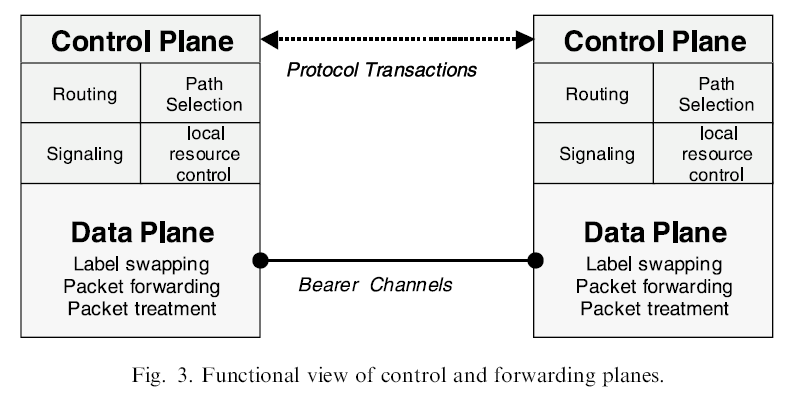
\includegraphics[scale=0.35]{label.png}
    \end{center}
  \end{figure}    
\end{frame}

\begin{frame}
  \frametitle{MPLS Fundamentals: MPLS Architecture}
  \begin{figure}[h]
    \begin{center}
      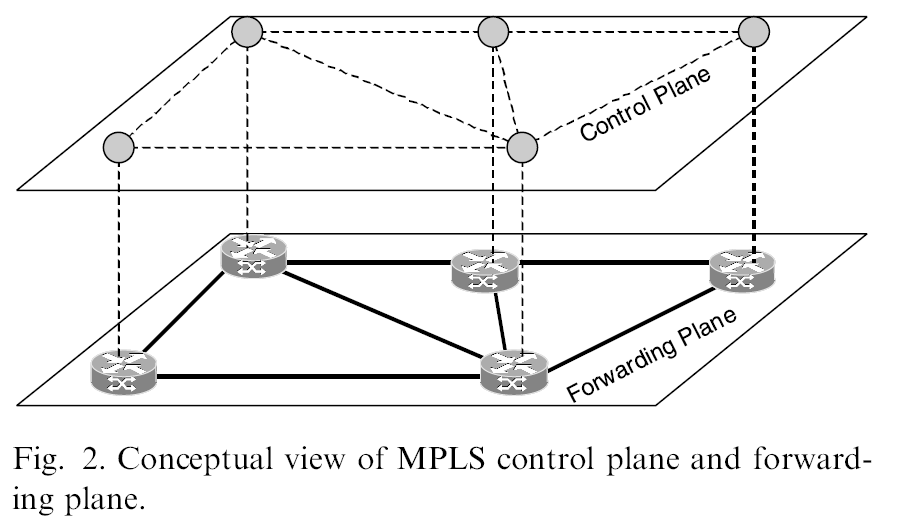
\includegraphics[scale=0.40]{separation.png}
    \end{center}
  \end{figure}
\end{frame}

\begin{frame}
  \frametitle{MPLS Fundamentals: Labels}
  \begin{itemize}
    \item A label is a short, fixed-length (4 bytes), header used to identify a FEC. The label on a packet represents the FEC for that packet.
    \item The label sits between data link layer header (Layer 2) and network layer header (Layer 3). They may be stacked, with the last label appearing last in the packet followed by the network layer packet. 
  \end{itemize}
  \begin{figure}[h]
    \begin{center}
      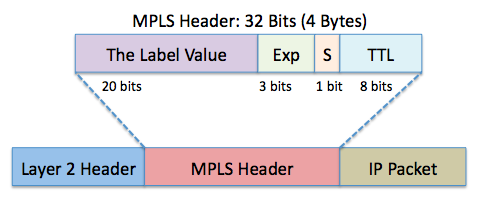
\includegraphics[scale=0.40]{header_mpls.png}
    \end{center}
  \end{figure}    
\end{frame}

\begin{frame}
  \frametitle{MPLS Fundamentals: The label header}
    \begin{itemize}
      \item {\bf{Label value: }}The label value. Label values 0-15 are reserved for specific tasks (for example: explicitly route based on IP packet header).
      \item {\bf{EXP field: }}"Experimental" bits now used as a Class of Service field for QoS (Diffserv).
      \item {\bf{Stack bit: }}Indicates that the bottom of the MPLS header stack has been reached.
      \item {\bf{Time-To-Live: }}Prevents looping in the MPLS network. This value decrements with each hop and packets are discarded if they have a zero value.
    \end{itemize}       
\end{frame}

\begin{frame}
  \frametitle{MPLS Fundamentals: Label switched paths}
  \begin{figure}
    \includegraphics<1>[scale=0.5]{animations/routeInit.png}
    \includegraphics<2>[scale=0.5]{animations/routereq1.png}
    \includegraphics<3>[scale=0.5]{animations/routereq2.png}
    \includegraphics<4>[scale=0.5]{animations/labeltable1.png}
    \includegraphics<5>[scale=0.5]{animations/labeltable2.png}
    \includegraphics<6>[scale=0.5]{animations/labeltable3.png}
    \includegraphics<7>[scale=0.5]{animations/labeltable4.png}
    \includegraphics<8>[scale=0.4]{animations/labeltable5.png}
    \includegraphics<9>[scale=0.4]{animations/path1.png}
    \includegraphics<10>[scale=0.4]{animations/path2.png}
    \includegraphics<11>[scale=0.4]{animations/path3.png}
    \caption{
      \only<1>{Initial state.}
      \only<2>{Ingress node requests a given destination address from the nearest node.}
      \only<3>{The request is routed to the destination node.}
      \only<4>{A MPLS switching table is initialized that says that all packets with a given label id are meant for router 47.1.}
      \only<5>{The mapping is sent back to the router we recieved the request from.}
      \only<6>{The router that receives the mapping, adds it to its switching table.}
      \only<7>{This continues until we reach the ingress node.}    
      \only<8>{When we reach the ingress node the given label switched path for that label will be complete.}
      \only<9>{A packet arrives that is headed for 47.1 and should use this LSP. The Ingress node makes a lookup in its switching table and assigns the correct label to the packet.}
      \only<10>{As the packet traverses the LSP labels are added, removed, or swapped as needed as the packet is forwarded from router to router.}
      \only<11>{When the packet has reached the egress node all labels are popped and the packet is delivered to the specified destination.}    
    }
  \end{figure}
\end{frame}

\begin{frame}
  \frametitle{Traffic Engineering}
  \begin{itemize}
    \item Traffic engineering deals with performance optimization of operational ip networks. We want to transport ip packets in the most efficent reliable and quick manner possible through a given network.
    \item To do this we want to avoid congestion and facilitate recovery when problems occur.
    \item We want to take advantage of alternative viable paths when there exists overutilized and congested resources and generally place traffic where the capacity exists to accommodate it.
    \item The ability to enable constraint-based routing in IP networks is one of the achievements of MPLS that makes it particularly useful for traffic engineering.
  \end{itemize}
\end{frame}

\begin{frame}
  \frametitle{Traffic Engineering: Process Model}
  Traffic engineering is an iterative and cyclic process divided into 4 phases. Interaction between the phases characterize major and minor workcycles as shown in this figure.
  \begin{figure}[h]
    \begin{center}
      \includegraphics[scale=0.25]{processmodel.png}
    \end{center}
  \end{figure}
\end{frame}

\begin{frame}
  \frametitle{Traffic Engineering: Policy formulation phase}
    Strategic approach:
    \begin{itemize}
      \item Careful planning of the LSP virtual topology.
      \item Systemated reconfiguration of LSPs.
      \item Forecast traffic patterns. Plan for future demands.
      \item Pay close attention to how, where, and when new LSPs are activated to address performance issues.
    \end{itemize}

    Tactical approach:
    \begin{itemize}
      \item Establish and manage explicit LSPs to address very specific network performance problems. Ad-hoc. Example: Create new LSPs to divert traffic away from congested network resources onto under-utilized alternatives.
      \item Also called "hybrid approach" because it involves using LSPs to control only some parts of the network while other segments are handled using regular routing protocol metrics.
    \end{itemize}
\end{frame}

\begin{frame}
  \frametitle{Traffic Engineering: Data acquisition phase}
    \begin{itemize}
      \item Monitor, measure and store various performance and fault statistics associated with LSPs and the network infrastructure.
      \item Traffic performance, resource utilization, measurement of routes used by specific traffic streams or between specified nodes.
      \item Essentially the feedback component of the traffic engineering process model.
    \end{itemize}
\end{frame}

\begin{frame}
  \frametitle{Traffic Engineering: Analysis and characterization phase}
    \begin{itemize}
      \item Analyze the information gained from the data acquisition phase and try to understand the root causes of unwanted network behavior.
      \item Can also identify hot-spots, peak-rates and seasonality in the network.
      \item Very complex, usually done offline, requires advanced mathematical models.
    \end{itemize}
\end{frame}

\begin{frame}
  \frametitle{Traffic Engineering: Performance optimization phase}
  Select best course of action to enchance network performance. This may involve:
    \begin{itemize}
      \item Creating new LSPs using an appropriate path selection mechanism.
      \item Reroute existing LSPs to reduce congestion or go around a networm problem.
      \item Tear down or deactivate an existing LSP that is causing problems.
      \item Modulate the behavior of existings LSPs or the network devices that they involve.
      \item Add additional capacity and/or expand the network topology.
      \item Create multiple new LSPs with the same endpoint and divide the traffic between them.
    \end{itemize}
\end{frame}

\begin{frame}
  \frametitle{Traffic Engineering: MPLS-based}
  MPLS is particularly suited for traffic engineering because:
    \begin{itemize}
      \item No need for an overlay network which reduces the amount of network devices needed and therefore operating costs.
      \item This also leads to greater reliability since there are fewer elements along the path where things may go wrong.
      \item Potentially less latency for the same reason.
      \item Simplified network architectures that are easier to manage.
      \item Better routing protocols and better estimates of the traffic matrix in our network.
    \end{itemize}
\end{frame}

\begin{frame}
  \frametitle{Traffic Engineering: Diffserv-aware}
  Differentiated services provide a coarse-grained mechanism for classifying network traffic and is used to provide QoS.
  \begin{itemize}
      \item Classification is done at the edge of the network and is then applied on a per hop basis.
      \item Up to 64 different classes possible, however we generally only use the default (best effort), expedited (low latency/low loss) or assured (delivered by prescribed conditions) PHBs.
      \item Combined with MPLS conditional routing we get even more fine grained control that can be used to prioritize traffic and strengthen guarantees.
      \item Allows ISPs to create class specific virtual networks with specified capacities.
      \item The Diff-Serv class can be defined either by the experimental bits in the MPLS header (EXP-inferred-LSP) or by label (Label-inferred-LSP). 
  \end{itemize}
\end{frame}

\begin{frame}
  \frametitle{Traffic Engineering: Challenges and considerations}
    \begin{itemize}
      \item Computation of paths for LSPs with constraints are complex operations and present us with a NP-complete problem.
      \item How do we deal with path restoration if we lose a critical network device. Should we have parallell paths ready to gracefully handle such instances?
      \item More LSPs allow us to optimize the network more effectily, but increase the operational complexity.
      \item Difficult for customers to gain insight into the MPLS cloud. How to monitor that your carrier is delivering the correct performance?
  \end{itemize}
\end{frame}

\begin{frame}
  \frametitle{GMPLS: What is GMPLS?}
  \begin{itemize}
    \item A protocol suite extending MPLS to serve as the control plane for other types of transport networks such as Time Division Multiplex networks and Optical transport networks.
    \item Provides uniform and consistent signaling, routing and link managment and advocates explicit separation of the control plane from the underlying data/forwarding plane.
    \item Extends the concept of a label so that a label can now also be a time slot in a TDM network, a wavelength in a wavelength-switched network or a fiber in a fiber-switched network.
  \end{itemize}
\end{frame}

\begin{frame}
  \frametitle{GMPLS: What else is new?}
  \begin{itemize}
    \item Decouples the control channel from the transport channel, but requires bi-diurectional control channels between nodes even though a connection might be unidirectional at the transport level.
    \item Introduces a plethory of new extentions to the conventional IP routing and traffic engineering protocols. Almost every aspect of the MPLS traffic engineering signaling protocols have been enhanced to support the GMLS concept.
    \item Failure indication mechanisms have been added to allow downstream nodes to notify upstream nodes of failures (no light) although a failure in the control plane does not neccesarily imply a failure in the transport plane.
  \end{itemize}
\end{frame}

\begin{frame}
  \frametitle{GMPLS: Why use GMPLS?}
  \begin{itemize}                             
    \item Allows new and innovative ways to inter-connect various technologies and different layers, without restricting the way individual layers interwork with each other. 
    \item Simplifies the design, deployment and operations management of heterogeneous networks consisting of an assortment of packet and circuit switched equipment from different manufacturers.
  \end{itemize}
\end{frame}

\begin{frame}
  \frametitle{Conclusion}
  \begin{itemize}                             
    \item This presentation describes some of the basic concepts of MPLS and GMPLS with specific attention paid to how they apply to traffic engineering.
    \item GMPLS will be an important parth of the next generation of computer networks with optical networks being the defacto standard for network infrastructure.
    \item New advances in technology will result in more changes to the way traffic engineering is performed and we might yet still see further extentions to the current set of IP technologies.  
  \end{itemize}
\end{frame}

\begin{frame}
  \frametitle{References and resources}
  \begin{itemize}
    \item Generalized Multiprotocol Label Switching: An Overview of Signaling Enhancements and Recovery Techniques
          IEEE Communication Magazine, July 2001.
          A. Banerjee et. al. 
    \item Internet Traffic Engineering Using Multi-Protocol Label Switching (MPLS).
          Computer Networks 40, Elsevier, 2002
          D.O. Awduche and B. Jabbari. 
    \item Dr. Denbanjan Saha for MPLS Label distribution teaching aid.
  \end{itemize}
\end{frame}
\end{document}
